\chapter{Harmonic Excitation}
\label{chap:Excitation}

\section{Introduction}
\label{sec:Excitation-Introduction}
	Nonlinear distortion is an inherent part of an analogue signal path. It alters the dynamic variation of signals and
	introduces new spectral components. Its use as a creative effect is best known by guitar players due to the use of
	valves in early guitar amplifiers imparting nonlinear transforms onto the audio signal
	\citep{dutilleux2011nonlinear}. This distorted sound became desirable and several electronic circuits were
	developed with the purpose of inducing nonlinear distortion. More recently, research into modelling these
	distortion circuits in the digital domain has been carried out, such as that done by \citet{pakarinen2009a}.
	Several researchers have also worked on creating novel digital distortion techniques
	\citep{fernandez-cid2001distortion, puckette2007patch, pekonen2008coefficient}.

	Historically, distortion is a very broad term which is often used to describe unwanted effects. For this work a
	more strictly defined term, harmonic excitation, will be used to refer to the deliberate and controlled application
	of nonlinear or time variant systems in order to introduce new frequency components to a signal.
	\citet{dutilleux2011nonlinear} defines excitation as the process of controlling timbre through the emphasis of
	certain frequencies. While this is possible with linear systems such as equalisers, nonlinear and time variant
	systems provide more flexibility as they can add energy in areas of the spectrum where the original signal had
	none.

	This chapter will review previous analysis of nonlinear systems as applied to audio processing, how their effects
	are quantified and the timbral transforms they impart. Firstly the analysis of nonlinear systems is discussed in
	Section~\ref{sec:Excitation-AnalysisOfNonlinearSystems}. Existing research into the perceived timbral effects of
	these systems is then discussed in Section~\ref{sec:Excitation-Timbre}. Section~\ref{sec:Excitation-Uses} describes
	the common uses for nonlinear distortion by audio engineers. Section~\ref{sec:Excitation-Methods} then explains the
	operation of various nonlinear systems used, or proposed for use, in audio processing.

\section{Analysis of Nonlinear Systems}
\label{sec:Excitation-AnalysisOfNonlinearSystems}
	The behaviour of an \acrshort{lti} system can be entirely summarised by its response to a unit impulse signal (the
	Kronecker delta function) \citep{phillips2007signals}. This is known as the system's impulse response, $A[n]$, and
	can be used to calculate the response of the system to an arbitrary input signal, $x[n]$, via convolution
	(Equation~\ref{eq:Convolution}).

	\begin{equation}
		y[n] = \sum_{m = 0}^{M - 1} A[m]x[n-m]
		\label{eq:Convolution}
	\end{equation}

	where $M$ is the length of the system's impulse response.
	
	Analysis of nonlinear systems is more complicated, unlike \acrshort{lti} systems the properties of the system
	cannot be summarised by the system's response to a single input signal. Depending on the field in which a nonlinear
	system is being studied, different approaches are taken in an attempt to summarise the behaviour of nonlinear
	systems. In the field of audio engineering, much of the literature concerning nonlinearities has to do with
	minimising distortion or measuring the maximum allowable levels of distortion. Several distortion metrics have been
	developed each with their own uses. A review of many of these metrics is given by \citet{voishvillo2006assessment},
	some of which will be discussed in Section~\ref{sec:Excitation-Analysis-Metrics}.  Where more information is
	needed, nonlinear modelling techniques are used.  These typically involve setting the parameters of a generalised
	nonlinear system such that its behaviour matches that of the system being analysed. The nonlinear modelling
	techniques utilised in the audio processing literature are discussed in
	Section~\ref{sec:Excitation-Analysis-Modelling}. Prior to discussing how the effects of nonlinear systems are
	measured / modelled, the concept of distortion components (the artefacts introduced by nonlinear systems) is
	introduced in Section~\ref{sec:Excitation-Analysis-Components}.

	\subsection{Distortion Components}
	\label{sec:Excitation-Analysis-Components}
		Nonlinear systems introduce new spectral components to a signal. These distortion components are produced
		via intermodulation of the existing spectral components in the signal. The frequencies of these distortion
		components are linear combinations of the frequency components in the input signal. For a signal with $N$
		frequency components the frequency, $\nu$, of each possible distortion component takes the form of
		Equation~\ref{eq:IntermodulationComponents} \citep{hulick2005solid}.

		\begin{equation}
			\nu = \sum_{n = 1}^{N} k_{n}\nu_{n}, \quad k_{n} \in \textbf{Z}
			\label{eq:IntermodulationComponents}
		\end{equation}

		where $\nu_{n}$ is the frequency of the $n$\super{th} frequency component of the input signal and each
		$k_{n}$ an integer scaling factor. The order of the distortion component, $O$, is calculated as the sum of
		the absolute values of these scaling factors (Equation~\ref{eq:IntermodulationOrder}).

		\begin{equation}
			O = \sum_{n = 1}^{N} \abs{k_{n}}
			\label{eq:IntermodulationOrder}
		\end{equation}

		The exact distortion components introduced are determined by the input signal and the system used to
		process it. The components introduced can be ascribed to two different groups: harmonic and intermodulation
		distortion.

		\subsubsection*{Harmonic Distortion}
			Harmonic distortion refers to the distortion components generated by a signal's frequency
			components modulating themselves. This refers to the situation where all but one of the scaling
			factors, $k_{n}$, in Equation~\ref{eq:IntermodulationComponents} are zero. The frequencies of every
			harmonic distortion component are integer multiples of a frequency component in the original
			signal. For a sinusoidal input only harmonic distortion components are generated. The number of
			harmonic distortion components introduced grows linearly with the number of frequency components in
			the input signal.

		\subsubsection*{Intermodulation Distortion}
			Intermodulation distortion refers to distortion components introduced when two or more of the
			spectral components in a signal modulate each other. If all the components in the input are
			harmonically related the intermodulation components will also lie at harmonic frequencies. A signal
			with slight inharmonicities in it will produce intermodulation components which amplify these
			inharmonicities. Due to this possible increase in inharmonicity, intermodulation distortion
			components are often considered to be less audibly pleasant than those of harmonic distortion
			\citep{rumsey2009sound}. The number of intermodulation components grows factorially as the number
			of frequency components in the input increases. This makes it more difficult to predict the
			intermodulation characteristics of a system for arbitrary input signals.

		\subsubsection*{Aliasing}
			In a digital system, continuous signals must be represented by discrete signals. This is achieved
			through sampling, each sample representing the amplitude of the original signal at a particular
			point in time. The number of samples of the signal's amplitude measured per second is referred to
			as the sampling frequency, $f_{s}$. The sampling frequency of a discrete signal imposes a
			restriction on the highest frequency which can be represented within it. This frequency is known as
			the Nyquist frequency, $f_{N}$, and is calculated using Equation~\ref{eq:nyquist}.

			\begin{equation}
				f_{N} = \frac{f_{s}}{2}
				\label{eq:nyquist}
			\end{equation}

			When sampling a signal, frequency content above $f_{N}$ is represented as aliased frequencies
			between 0Hz and $f_{N}$. The alias frequency, $f_{\mathrm{alias}}$, for a given frequency in the
			input signal, $f$, is the displacement between it and the nearest integer multiple of the sampling
			frequency (Equation~\ref{eq:aliasing}).

			\begin{equation}
				f_{\mathrm{alias}} = \abs{f - f_{s}\round{\frac{f}{f_{s}}}}
				\label{eq:aliasing}
			\end{equation}

			The new frequency content introduced to a discrete signal via nonlinear processing is also subject
			to aliasing. This can cause problems when predicting the behaviour of a nonlinear system in
			different scenarios, as the spectral content introduced will depend on the sampling frequency of
			the signal being processed. Thus, the perceived timbral transform may also depend on the sampling
			frequency. Steps can be taken to reduce the impact of aliasing on the performance of nonlinear
			effects; for example \citep{vetter2013estimation} describe a method for use with nonlinearities
			which produce harmonics whose amplitudes decrease as their frequencies increase. They upsample
			signals by a factor of 32 prior to applying nonlinear processing; this endures that only the low
			amplitude, high frequency partials are aliased. If the upsampling factor is sufficiently high these
			aliased partials will be rendered inaudible. After processing the signal is downsampled to the
			original sampling frequency. Upsampling increases the computational complexity of a system, along
			with the extra overhead of upsampling and downsampling the signal there is also a larger number of
			samples to process. For certain excitation methods it may be possible to reduce aliasing by
			changing properties of the processing algorithm. Details of these techniques will be discussed
			where appropriate in Section~\ref{sec:ExcitationEvaluation-Comparison}.

	\subsection{Objective Distortion Metrics}
	\label{sec:Excitation-Analysis-Metrics}
		\subsubsection*{Traditional Metrics}
			Traditional measurements of the effects of nonlinear systems measure the ratio between the levels
			of unwanted distortion components and wanted frequency components in the output signal. Two
			metrics, \acrfull{thd} and \acrfull{imd}, are the traditional objective measures of distortion in
			audio systems \citep{czerwinski2001multitone1}. \acrshort{thd} measures the level of harmonic
			distortion components introduced by a system for a sinusoidal input signal and is calculated using
			two different methods. These have been denoted $\mathrm{THD}_{F}$ and $\mathrm{THD}_{R}$ by
			\citet{shmilovitz2005on} and are calculated using Equations \ref{eq:thdf} and \ref{eq:thdr}
			respectively.

			\begin{equation}
				\mathrm{THD}_{F} = \frac{\sqrt{\sum_{n = 2}^{\infty} h_{n}^{2}}}{h_{1}}
				\label{eq:thdf}
			\end{equation}

			\begin{equation}
				\mathrm{THD}_{R} = \sqrt{\frac{\sum_{n = 2}^{\infty} h_{n}^{2}}
								       {\sum_{n = 1}^{\infty} h_{n}^{2}}}
				\label{eq:thdr}
			\end{equation}

			where $h_{n}$ is the amplitude of the $n$\super{th} harmonic. 

			Each of these measures has slightly different properties. $\mathrm{THD}_{F}$ measures the relative
			levels of new harmonic content and the energy at the frequency of the original sinusoid, producing
			a positive value. $\mathrm{THD}_{R}$ measures the proportion of the output signal which consists of
			new harmonic components, producing a value between zero and one. \citet{shmilovitz2005on} suggests
			that $\mathrm{THD}_{F}$ provides a better measure for signals with high distortion as there is no
			upper bound on the value which is produced.  Both methods have been used in recent work published
			in the audio processing field ($\mathrm{THD}_{F}$ by \citet{fleischmann2014a} and
			$\mathrm{THD}_{R}$ by \citet{dutilleux2011nonlinear}).  The lack of standardisation for this metric
			makes it difficult to compare experimental results reported by different sources.

			Various standards exist for the measurement of \acrshort{imd}. Typically the system's response to a
			signal consisting of two sinusoids is measured. According to the \citet{IEC2001amplifiers}
			standard, a signal comprising two frequency components, $f_{1}$ and $f_{2}$ (where $f_{2} >
			f_{1}$), with an amplitude ratio of 4:1 is used.  The levels of the second and third order
			intermodulation components present in the output is then measured separately according to Equations
			\ref{eq:imd2} and \ref{eq:imd3}.

			\begin{equation}
				\mathrm{IMD}_{2} = 100\frac{a_{f_{2} + f_{1}} + a_{f_{2} - f_{1}}}{a_{f_{2}}}
				\label{eq:imd2}
			\end{equation}

			\begin{equation}
				\mathrm{IMD}_{3} = 100\frac{a_{f_{2} + 2f_{1}} + a_{f_{2} - 2f_{1}}}{a_{f_{2}}}
				\label{eq:imd3}
			\end{equation}

			where $a_{f}$ is the amplitude of frequency $f$ in the output signal.

			\acrshort{thd} and \acrshort{imd} give very limited information about the response of nonlinear
			systems. They are typically measured using simple input signals which are not representative of the
			signals a system would process in actual use. Given that nonlinear systems do not satisfy the
			condition of superposition, a system may process simple and complex signals in vastly differing
			manners. These metrics also give no indication of the perceived degradation in audio quality a
			system introduces.  A signal with a high \acrshort{thd} value may potentially sound less distorted
			than one with a small \acrshort{thd}. To measure the perceived levels of distortion a system
			produces, metrics which are based around psychoacoustic principles are required.

		\subsubsection*{Psychoacoustically Influenced Metrics}
			Several researchers have developed new distortion metrics which indicate the perceived amount of
			distortion. \citet{geddes2003auditory} suggest three psychoacoustic principles which may be
			applicable to the analysis of nonlinear distortion:

			\begin{itemize}
				\item New frequency components introduced, with lower frequencies than the original
					components, will be more perceptible.
				\item Higher order distortion components will be more perceptible.
				\item Nonlinearities which affect lower amplitude signals will be more perceptible.
			\end{itemize}

			\citet{voishvillo2006assessment} adds that the perception of distortion is decreased at the very
			high and low ends of the frequency spectrum.

			A subset of nonlinear systems can be described by a characteristic curve (a function mapping the
			instantaneous amplitude of the input signal to the amplitude of the output signal). These systems
			are referred to as static nonlinearities and are memoryless systems (their behaviour is only
			governed by the instantaneous amplitude of the input, not any of its previous states). The GedLee
			metric, $G$, proposed by \citet{geddes2003auditory}, measures the level of audible distortion
			produced by a static nonlinearity through analysis of its characteristic curve, $T(x)$. It is
			calculated using Equation~\ref{eq:gedlee}.

			\begin{equation}
				G = \sqrt{\int_{-1}^{1} \left( \cos \left( \frac{x\pi}{2} \right) \right)^{2}
					      \left( \frac{d^{2}}{dx^{2}} T(x) \right)^{2} dx}
				\label{eq:gedlee}
			\end{equation}

			A considerable advantage of the GedLee metric is that it directly measures the system in question
			rather than signals processed by it. This should allow measurements taken using the metric to
			describe the audible degradation of any signal processed by a system. In a second paper,
			\citet{lee2003auditory} provide results of an experiment in which their metric was tested against
			\acrshort{thd} and \acrshort{imd} as a rating of audio quality. They show that for low levels of
			distortion the GedLee metric correlates with subjective audio quality ratings. \acrshort{thd} and
			\acrshort{imd} are both found not to correlate well with perceived quality. The GedLee metric is
			only applicable to the analysis of static nonlinearities. Many nonlinear systems are more complex
			than this and may exhibit frequency dependent or time variant behaviour. While the GedLee metric
			may provide a good, signal independent, measure of distortion, it is only applicable to a subset of
			nonlinear systems.

			\citet{tan2003the} also developed a perceptual metric for distortion, Distortion Score
			($\mathrm{DS}$), which employs models of the human hearing system to better approximate the
			perceived level of distortion. Firstly, both the input and output signal of the system under test
			are split into $I$ non-overlapping frames, each 30ms long. Then the spectrum of each frame is
			calculated using the \acrshort{dft}. The frequency selectivity of the human hearing system is taken
			into account by splitting the spectrum of each frame into $J$ non-overlapping bands which are each
			one \acrshort{erb} in width. The final distortion score, $\mathrm{DS}$, is calculated from the
			difference in power between these bands in the input and output signal according to
			Equation~\ref{eq:DistortionScore}.

			\begin{gather}
				\mathrm{IP}_{i,j} = \sum_{n = 1}^{N_{j}} X_{i,j}^{2}[n] \nonumber \\
				\mathrm{OP}_{i,j} = \sum_{n = 1}^{N_{j}} Y_{i,j}^{2}[n] \nonumber \\
				\mathrm{DS} = \frac{1}{I} \sum_{i = 1}^{I} \sum_{j = 1}^{J} 
					\abs{10\log_{10} \left( \frac{\mathrm{OP}_{i,j}}{\mathrm{IP}_{i,j}} \right) }
				\label{eq:DistortionScore}
			\end{gather}

			where $X_{i,j}[n]$ and $Y_{i,j}[n]$ are the $j$\super{th} band of the spectra of the $i$\super{th}
			frame of the input and output signals respectively and $N_{j}$ the number of spectral bins in that
			band.
			
			\citet{tan2004predicting} suggest improvements to the $\mathrm{DS}$ metric leading to the
			$R_{\mathrm{nonlin}}$ metric. The first improvement is the inclusion of a filter with a frequency
			response similar to that of the outer and middle ear. The filter used is described by
			\citet{glasberg2002a}, it attenuates frequencies at either end of the audible spectrum, modelling
			the decreased perception of distortion at these frequencies as reported by
			\citet{voishvillo2006assessment}. The calculation of $R_{\mathrm{nonlin}}$ is split into several
			steps as follows:
			
			\begin{enumerate}
				\item A signal, $x[n]$, is processed by the system under test producing an output signal,
					$y[n]$.

				\item $x[n]$ and $y[n]$ are time aligned and each filtered using the outer and middle ear
					filter discussed previously.

				\item The signals are then processed by a parallel bank of 40 gammatone filters each one
					\acrshort{erb} wide. The input and output signals processed by gammatone filter $j$
					are denoted $x_j[n]$ and $y_j[n]$ respectively.

				\item The outputs of each gammatone filter are then split into non-overlapping 30ms frames
					and the normalised cross-correlation between the input and output frame is
					measured.  To account for any frequency dependent delay introduced by the system
					under test, a variable lag parameter, $\tau$, is introduced to offset the input and
					output signals from one another in time. For each frame, $i$, band, $j$, and lag
					value, $\tau$, the normalised cross-correlation between the input and output
					signals, $r_{i,j,\tau}$, is calculated using
					Equation~\ref{eq:RNonlinCrossCorrelation}.

					\begin{gather}
						S_{i,\tau} = \left\{ n | n \in \textbf{Z} 
							   \land (i-1)L+\tau+1 \leq n \leq iL + \tau \right\} \nonumber \\
						r_{i,j,\tau} = \frac{\sum_{n \in S_{i,\tau}} x_{j}[n]y_{j}[n-\tau]}
							{\left( \sum_{n \in S_{i,\tau}} x_{j}^{2}[n] \right) 
							\left( \sum_{n \in S_{i,\tau}} y_{j}^{2}[n-\tau] \right)}
						\label{eq:RNonlinCrossCorrelation}
					\end{gather}

					where $S_{i,\tau}$ is the range of samples from the input signal used in the
					calculation, given the frame number and the value of the lag parameter; and $L$ is
					the number of samples in a 30ms frame, given the sampling frequency ($L =
					\round{0.03f_{s}}$). 

				\item For each frame and band the maximum value of this cross-correlation, $M_{i,j}$, is
					found for lag times at one sample increments between -10ms and 10ms
					(Equation~\ref{eq:RNonlinMaxCrossCorrelation}).

					\begin{gather}
						\mathrm{T} = \round{0.01f_{s}} \nonumber \\
						M_{i,j} = \max_{\tau = -\mathrm{T}}^{\mathrm{T}} r_{i,j,\tau}
						\label{eq:RNonlinMaxCrossCorrelation}
					\end{gather}

				\item The values of $M_{i,j}$ are then weighted according to the power present in the
					relevant frame and band of the output signal, $P_{i,j}$, and the maximum power of
					all bands in that frame, $Q_{i}$. The weighting for each band and frame, $W_{i,j}$
					is calculated using Equation~\ref{eq:RNonlinWeighting}.

					\begin{gather}
						P_{i,j} = 10\log_{10} \left( \frac{1}{L} 
							\sum_{n=(i-1)L+1}^{iL} y_{j}^{2}[n]\right) \nonumber \\
						Q_{i} = \max_{j = 1}^{40} P_{i,j} \nonumber \\
						W_{i,j} = \begin{cases}
							1 & \text{if $Q_{i} - P_{i,j} \leq 40$} \\
							\frac{P_{i,j} - Q_{i} + 80}{40} & 
								\text{if $40 < Q_{i} - P_{i,j} \leq 80$} \\
							0 & \text{otherwise} \\
						\end{cases}
						\label{eq:RNonlinWeighting}
					\end{gather}

					This weighting ensures that only bands which contain sufficient energy contribute
					to the final distortion metric. Prior to being applied the weights are normalised
					such that the sum of the weights for each frame is equal to 1 giving the normalised
					weights, $W'_{i,j}$, using Equation~\ref{eq:RNonlinWeightsNormalisation}.

					\begin{equation}
						W'_{i,j} = \frac{W_{i, j}}{\sum_{k = 1}^{40} W_{i,k}}
						\label{eq:RNonlinWeightsNormalisation}
					\end{equation}

				\item The final metric, $R_{\mathrm{nonlin}}$, is then calculated by summing across all 40
					bands and averaging across all $I$ frames using Equation~\ref{eq:RNonlin}.

					\begin{equation}
						R_{\mathrm{nonlin}} = \frac{1}{I} \sum_{i = 1}^{I} \sum_{j = 1}^{40} 
									W'_{i,j}M_{i,j}
						\label{eq:RNonlin}
					\end{equation}

			\end{enumerate}

			\citet{tan2004predicting} report greater correlation between $R_{\mathrm{nonlin}}$ and perceived
			audio quality then \citet{lee2003auditory} do for the GedLee metric. They also demonstrate how
			accurate the $R_{\mathrm{nonlin}}$ metric is in predicting the perceived distortion level
			introduced to music and speech signals. However, both $\mathrm{DS}$ and $R_{\mathrm{nonlin}}$ rely
			on analysing signals which have been processed by the system under test so they may not give
			results which can be applied as generally as those using the GedLee metric.

			The metrics discussed in this section provide one dimensional measurements of some aspect of a
			nonlinear system, be it the proportion of the output signal which is made up of a particular type
			of distortion component or a more advanced metric which measures the perceived amount of audio
			degradation a system causes. These can be useful for summarising the distortion characteristics of
			a system but in many cases may not be sufficient to fully describe the operation of a system. A
			more comprehensive approach is to model the operation of a nonlinear system using a template system
			with multiple parameters.

	\subsection{Nonlinear Modelling}
	\label{sec:Excitation-Analysis-Modelling}
		Various techniques for modelling nonlinear systems have been proposed and developed in the fields of
		mathematics and engineering. These models allow for more in depth analysis of a nonlinear system as well as
		replicating its effects in the digital domain. Summaries of some of these modelling techniques can be found
		in the work by \citet{janczak2005identification} and \citet{ogunfunmi2007adaptive}. Three of these models
		that have been used to model the operation of nonlinear audio effects are described in the following
		sections.

		%\begin{itemize}
		%	\item Wave Digital Filters
		%	\item Volterra Series
		%	\item The Synchronised Swept Sine Method
		%\end{itemize}

		%These techniques are summarised here.

		\subsubsection{Wave Digital Filters}
			Wave digital filters are a class of filter which can be used to emulate analogue circuits. The
			process of creating a digital representation of a circuit involves constructing a `tree' of blocks.
			These blocks represent either electronic components, or connections between components in a
			circuit.  Each block obeys a certain set of rules when presented with a signal as described by
			\citet{fettweis1986wave}. Blocks have been developed for modelling nonlinear circuit elements such
			as operational amplifiers and diodes \citep{paiva2012emulation}.

			While wave digital filters can accurately represent a nonlinear system, there are some
			disadvantages. As systems get more complex, traversing the `tree' of blocks in order to calculate
			the output signal takes more computation. This presents problems when real time system response is
			needed. There are also certain circuit topologies which cannot be represented in the wave digital
			domain \citep{valimaki2011virtual}. Another consideration is that knowledge of the circuitry of the
			system being modelled is needed. This might not always be available.

		\subsubsection{Volterra Series}
			Modelling a nonlinear system using a Volterra series can be considered an extension of modelling an
			\acrshort{lti} system by measuring its impulse response. The response of the system to a
			pseudo-random test signal is used to calculate a series of kernels using methods described by
			\citet{schetzen1980the}.  These Volterra kernels are analogous to an \acrshort{lti} system's
			impulse response and can be used to calculate the output of the system to an arbitrary input using
			Equation~\ref{eq:VolterraSeries} (shown graphically in Figure~\ref{fig:VolterraModel}).

			\begin{equation}
				y[n] = g_{0} + \sum_{p = 1}^{P} 
					\sum_{m_{1} = 0}^{M - 1} \dotsi \sum_{m_{p} = 0}^{M - 1}
					g_{p}[m_{1}, \dotsc , m_{p}]
					\prod_{j = 1}^{p} x[n - m_{j}]
				\label{eq:VolterraSeries}
			\end{equation}

			where $P$ is the order of the Volterra series and $g_{p}[m_{1}, \dotsc , m_{p}]$ is the
			$p$\super{th} order Volterra kernel. The order of a Volterra kernel defines its dimensionality,
			$g_{0}$ being a constant, $g_{1}[m_{1}]$ being a one dimensional array of length $M$, $g_{2}[m_{1},
			m_{2}]$ being an $M \times M$ two dimensional array and so on. When $P = 1$ the Volterra series is
			equivalent to convolution by $g_{1}[m_{1}]$ and a DC offset by $g_{0}$.

			\begin{figure}[h!]
				\centering
				\begin{tikzpicture}
					\node (Kernel0) at (4, 3) {$g_{0}$};
					\node (Kernel1) [draw] at (1.5, 3) {$g_{1}[m_{1}]$};
					\node (Kernel2) [draw] at (1.5, 2) {$g_{2}[m_{1}, m_{2}]$};
					\node (KernelN) [draw] at (1.5, 0.5) {$g_{P}[m_{1}, \dotsc , m_{P}]$};

					\draw [dots] (Kernel2) -- (KernelN);

					\coordinate (Out1) at (3.5, 3);
					\coordinate (Out2) at (3.5, 2);
					\coordinate (OutN) at (3.5, 0.5);

					\draw (Kernel1) -- (Out1);
					\draw (Kernel2) -- (Out2);
					\draw (KernelN) -- (OutN);

					\node (Add) [operator] at (4, 1.75) {+};
					\draw (Kernel0) -- (Add);
					\draw (Out1) -- (Add);
					\draw (Out2) -- (Add);
					\draw (OutN) -- (Add);

					\coordinate (In1) at (-0.5, 3);
					\coordinate (In2) at (-0.5, 2);
					\coordinate (InN) at (-0.5, 0.5);

					\draw (In1) -- (Kernel1);
					\draw (In2) -- (Kernel2);
					\draw (InN) -- (KernelN);
					\draw (InN) -- (In1);

					\node (In) at (-1.25, 1.75) {$x[n]$};
					\coordinate (InMid) at (-0.5, 1.75);
					\draw (In) -- (InMid);

					\node (Out) at (5, 1.75) {$y[n]$};
					\draw (Add) -- (Out);

				\end{tikzpicture}
				\caption{A graphical depiction of the application of a Volterra series. Each of the
					rectangular boxes represents processing by the $p$\super{th} order Volterra
					kernel.}
				\label{fig:VolterraModel}
			\end{figure}

			Unlike wave digital filters, modelling a nonlinear system using a Volterra series requires no prior
			knowledge about the operation of the system. The Volterra kernels are calculated by the system's
			response to a predefined signal. Despite this, not all nonlinear systems can be modelled using a
			Volterra series. Much like a linear impulse response the Volterra series is only able to model time
			invariant systems. Other properties a system must exhibit in order to allow Volterra series
			modelling are discussed by \citet{billings2013nonlinear}.

			The use of Volterra series is computationally demanding, as the order of the series used increases
			the number of coefficients in the kernels rises exponentially. This can make the use of high order
			systems impractical. \citet{reed1996practical} suggests a method by which the number of
			coefficients can be reduced in the implementation of Volterra series to combat this.

		\subsubsection{The Synchronised Swept Sine Method}
			The synchronised swept sine method is another technique by which a nonlinear system can be modelled
			without prior knowledge of its operation. A series of impulse responses are generated by analysing
			the system's response to a signal with exponentially increasing frequency as described by
			\citet{novak2010nonlinear}. These impulse responses can then be used to calculate the output of the
			system to an arbitrary input using Equation~\ref{eq:HammersteinSeries}.

			\begin{equation}
				y[n] = \sum_{p = 1}^{P}
					\sum_{m = 0}^{M - 1} A_{p}[m]x^{p}[n-m]
				\label{eq:HammersteinSeries}
			\end{equation}

			This is a generalised polynomial Hammerstein system of order $P$ where $A_{p}[m]$ is the
			$p$\super{th} impulse response. The model is, in effect, an extension of a Taylor series of order
			$P$. The input is raised to each individual power, 1 through $P$, and each of these signals is
			convolved by an individual impulse response, $A_{p}[m]$. The resultant signals are then summed to
			produce the output. This is shown graphically in Figure~\ref{fig:HammersteinModel}.

			\begin{figure}[h!]
				\centering
				\begin{tikzpicture}
					\node (Sig2) [draw] at (1, 3) {$x^{2}[n]$};
					\node (Sig3) [draw] at (1, 2) {$x^{3}[n]$};
					\node (SigN) [draw] at (1, 0.5) {$x^{p}[n]$};

					\node (Filter1) [draw] at (3, 4) {$A_{1}[m]$};
					\node (Filter2) [draw] at (3, 3) {$A_{2}[m]$};
					\node (Filter3) [draw] at (3, 2) {$A_{3}[m]$};
					\node (FilterN) [draw] at (3, 0.5) {$A_{p}[m]$};

					\draw (Sig2) -- (Filter2);
					\draw (Sig3) -- (Filter3);
					\draw (SigN) -- (FilterN);

					\draw [dots] (Sig3) -- (SigN);
					\draw [dots] (Filter3) -- (FilterN);

					\coordinate (Out1) at (4.5, 4);
					\coordinate (Out2) at (4.5, 3);
					\coordinate (Out3) at (4.5, 2);
					\coordinate (OutN) at (4.5, 0.5);

					\draw (Filter1) -- (Out1);
					\draw (Filter2) -- (Out2);
					\draw (Filter3) -- (Out3);
					\draw (FilterN) -- (OutN);

					\node (Add) [operator] at (5, 2.25) {+};
					\draw (Out1) -- (Add);
					\draw (Out2) -- (Add);
					\draw (Out3) -- (Add);
					\draw (OutN) -- (Add);

					\coordinate (In1) at (-0.5, 4);
					\coordinate (In2) at (-0.5, 3);
					\coordinate (In3) at (-0.5, 2);
					\coordinate (InN) at (-0.5, 0.5);

					\draw (In1) -- (Filter1);
					\draw (In2) -- (Sig2);
					\draw (In3) -- (Sig3);
					\draw (InN) -- (SigN);
					\draw (InN) -- (In1);

					\node (In) at (-1.25, 2.25) {$x[n]$};
					\coordinate (InMid) at (-0.5, 2.25);
					\draw (In) -- (InMid);

					\node (Out) at (6, 2.25) {$y[n]$};
					\draw (Add) -- (Out);

				\end{tikzpicture}
				\caption{The generalised polynomial Hammerstein model.}
				\label{fig:HammersteinModel}
			\end{figure}

			As with a Volterra series this method can be used to analyse `black box' systems where no prior
			information about their operation is known. A considerable advantage over the Volterra series is
			that all the impulse responses are one dimensional, meaning that higher order systems are more
			practical to implement. There are some disadvantages however. Firstly, there is no account for the
			dependence of the system on the amplitude of the input signal. This is shown by
			\citet{novak2010analysis} who demonstrate how two different circuits are emulated with different
			degrees of accuracy. There is also no definitive way of deciding what order Hammerstein model to
			use prior to testing.

\section{Timbre of Nonlinear Distortion}
\label{sec:Excitation-Timbre}
	The research, discussed thus far in this chapter, has focussed on measuring the extent to which unwanted distortion
	can be perceived, or on modelling the operation of a nonlinear system. This does not provide sufficient information
	for the description of the timbral effect of nonlinear systems. The listening tests performed by
	\citet{lee2003auditory} and \citet{tan2004predicting}, to verify the distortion metrics discussed, asked subjects
	to rate the quality of audio stimuli. It is possible that nonlinear distortion could alter the timbre of audio
	without deteriorating its perceived quality. To investigate this, experiments must be conducted in which
	participants are asked to rate the timbral characteristics of nonlinearly processed stimuli. This section reviews
	literature published in that regard.

	There is a wealth of research into how low level audio features influence timbre, as discussed in
	Chapter~\ref{chap:Timbre}. The mappings between low level features and semantic features from the literature can be
	applied to harmonic excitation effects, provided the excitation method used can influence the required low level
	features.  It is possible that there are semantic terms used to describe the timbre of nonlinear distortion which
	are seldom used to describe other timbres. The majority of timbral research does not focus on nonlinear distortion
	and as such does not highlight these semantic terms. There have been some publications specifically discussing the
	timbral effects of nonlinear distortion, their findings are discussed in this section.

	\citet{marui2005predicting} suggest that one of the primary outcomes of nonlinear distortion is the moving of
	spectral energy between low and high frequencies. They propose that aspects of this effect correlate with the
	descriptors: sharpness and brightness. In order to discover other timbral properties of nonlinear distortion they
	performed listening tests in which distorted guitar stimuli were assessed. The stimuli were each processed with
	different nonlinear systems and then further processed so that they had matching Zwicker Sharpnesses (an objective
	measure of sharpness \citep{fastl2007psychoacoustics} discussed in
	Section~\ref{sec:Timbre-TimbralFeatures-Sharpness}). This sharpness matching was done so that the difference in
	timbre not related to sharpness could be more easily observed. During the listening tests subjects were asked to
	rate the dissimilarity of stimuli presented in pairs. They were also asked to grade each individual stimulus on the
	bipolar adjective scales shown in Table~\ref{tab:distortionDescriptors}.

	\begin{table}[h!]
		\centering
		\begin{tabular}{|c|C{3cm}cC{3cm}|}
			\hline
			\bf{No.} & \multicolumn{3}{|c|}{\bf{Adjectives}} \tabularnewline
			\hline
			\hline
			1 & dark & $\Longleftrightarrow$ & bright \tabularnewline
			\hline
			2 & rough & $\Longleftrightarrow$ & smooth \tabularnewline
			\hline
			3 & diffuse & $\Longleftrightarrow$ & compact \tabularnewline
			\hline
			4 & thin & $\Longleftrightarrow$ & thick \tabularnewline
			\hline
			5 & sharp & $\Longleftrightarrow$ & dull \tabularnewline
			\hline
			6 & light & $\Longleftrightarrow$ & heavy \tabularnewline
			\hline
			7 & hard & $\Longleftrightarrow$ & soft \tabularnewline
			\hline
			8 & clear & $\Longleftrightarrow$ & muddy \tabularnewline
			\hline
			9 & clamorous & $\Longleftrightarrow$ & calm \tabularnewline
			\hline
			10 & strong & $\Longleftrightarrow$ & weak \tabularnewline
			\hline
			11 & uncomfortably loud & $\Longleftrightarrow$ & comfortable \tabularnewline
			\hline
		\end{tabular}
		\caption{Bipolar adjectives scales used by \citet{marui2005predicting} to assess the perception of
		         distortion.}
		\label{tab:distortionDescriptors}
	\end{table}

	Their results suggest that the differences between different nonlinearities can be described by `thickness' and, to
	a lesser extent, `diffuseness'. These results are also found by a second experiment in which a triadic comparison
	method is used to assess the dissimilarities between stimuli \citep{marui2005constructing}. Both these experiments
	were conducted in Japanese and the descriptors were translated to English for publication. The descriptors were
	initially chosen during an experiment by \citet{martens2002relating}. From this experiment it was shown that
	speakers of Japanese and speakers of Sinhalese disagree on how these terms are used to describe timbre. It is
	expected that there will be similar differences in presenting the translated descriptors to English speakers.

	\citet{tsumoto2015investigating} use factor analysis to identify two factors describing the timbre of distorted
	guitar sounds: `activeness' correlating with attack time and the spectral centroid in the first 30ms of the sound
	and 'brightness' correlating with the spectral centroid after the first 30ms. Various bipolar adjective scales are
	assigned to these factors, `activeness' being described as 'light $\Leftrightarrow$ heavy' and `weak
	$\Leftrightarrow$ strong' and `brightness' being described as `bright $\Leftrightarrow$ dark' and `dull
	$\Leftrightarrow$ sharp'. They also use the term `crunch' to describe sounds with a moderate amount of distortion.
	No evidence is provided that this terminology is used by a wide range of guitar players, it is merely the language
	used to discriminate certain distortion effects from each other in their paper.
	
	In a second paper \citep{tsumoto2016the} the same authors investigate the relationship between the `brightness' and
	Zwicker sharpness of distorted guitar signals. They show that for a given parameter setting on a distortion effect,
	the function describing the relationship between the perceived `brightness' and Zwicker sharpness of output signals
	is monotonically increasing. As the parameter of the effect is changed the number of distortion components
	introduced to the signal is changed. Conversely to their predictions, it is shown that if the output signals are
	processed to have matching Zwicker sharpnesses, those to which greater levels of distortion had been introduced
	were perceived to be less `bright' then those which were less distorted. This is explained by examining the
	relative levels of different orders of distortion components in the output, suggesting that the perception of
	distortion depends on the individual levels of different orders of distortion components.

	\citet{wilson2014characterisation} use a different approach to describe the distortion characteristics of popular
	music tracks. A panel of expert listeners rated several stimuli on two scales: distortion level and distortion
	character (hard or soft). These results were then used to train a classifier for identifying distortion character,
	various features of the signal's probability mass function being found to best characterise distortion. The stimuli
	were then used in a listening test in which participants were asked to choose words which describe the audio
	quality of the stimuli. The most often used word was `distorted', being used to describe the stimuli which were
	classified has having high distortion levels, suggesting that the concept of distortion is well known to listeners.
	The other descriptors elicited (`punchy', `clear', 'harsh' etc.) did not correlate well with any particular group
	of stimuli as categorised by the classifier. This may be to do with the method by which the original stimuli were
	classified by the expert panel; the descriptors which did not correlate may refer to perceptual dimensions other
	than distortion level and character. Training the classifier to only discriminate stimuli in these two dimensions
	removes any information about where the stimuli lie on these additional dimensions.

	From discussion of the previous literature it is apparent that the use of nonlinear systems contribute to a variety
	of aspects of timbre. Distortion effects are widely used as a creative tool in popular music production but the
	language used to describe their application differs across groups of people. The term `distorted' is used to
	describe the timbre of signals which have undergone distortion but does not allow for discrimination between the
	timbres of two distorted signals. The other descriptors used in the literature are correlated with features of a
	system's output signal rather than features of the nonlinearity itself. This warrants a need for harmonic
	excitation systems which give control over specific features of the output rather than just the parameters of the
	underlying nonlinearity. 

\section{Uses of Harmonic Excitation}
\label{sec:Excitation-Uses}
	While harmonic excitation algorithms are best known as a creative effect used by guitarists, they find use in
	several other areas of audio processing; these areas are summarised in Sections
	\ref{sec:Excitation-Uses-Reconstruction} through \ref{sec:Excitation-Uses-Enhancement}. While popular creative
	distortion algorithms are based on simple analogue electronic circuits, algorithms designed for these applications
	provide more control over the output signal in order to achieve their respective tasks.

	\subsection{High Frequency Reconstruction}
	\label{sec:Excitation-Uses-Reconstruction}
		In digital systems it can be beneficial to reduce the amount of data needed to represent an audio signal.
		This is done either to reduce the storage space needed or reduce the data rate required to transmit a
		signal. As a higher data rate is needed to represent high frequencies, these frequencies are removed during
		the data compression process. A lot of research has been carried out to develop methods by which these high
		frequencies can be estimated during the decompression process. This allows for the bandwidth to be
		constricted for storage or transmission but the full bandwidth to be restored when required.

		When compressing audio data using lossy audio codecs, the original signal, along with its high frequency
		components, is available before compression is applied. Parameters describing the high frequency content of
		the signal can be recorded and used to aid in the reconstruction of the high frequencies later
		\citep{dietz2002spectral, friedrich2007spectral}. The high frequency content is estimated from the low
		frequency information and then further shaped using these parameters. This leads to a distinction between
		`blind' and `non-blind' methods for reconstructing the high frequencies. A `blind' method uses only the
		information present in the low frequency signal, whereas `non-blind' methods make use of recorded
		parameters to increase the accuracy of the reconstruction. In the literature several methods for
		reconstruction of the higher frequencies are suggested:

		\begin{itemize}
			\item Through the use of a nonlinear device \citep{larsen2002efficient, sha2010high}.
			\item Spectral replication \citep{nagel2010a}, essentially shifting the spectrum into a higher
			      frequency band.
			\item Spectral folding \citep{friedrich2007spectral}, creating a mirror image of the existing
			      spectrum around the highest frequency.
			\item Spectral stretching \citep{nagel2009a}, stretching the existing spectrum to the desired
			      bandwidth.
		\end{itemize}

		These methods could be utilised in creative audio effects; they all introduce new harmonic spectral
		components which may enhance perceptual attributes of a sound. In this situation there is not any
		information about how the higher harmonics might behave, so the system will have to operate `blindly'. It
		is worth noting that when using these methods as creative audio effects, the objective is not to try to
		replicate high frequency content which is missing but to generate new high frequency content. The accuracy
		lost through using `blind' bandwidth extension methods is not a great concern for creative timbral
		manipulation work as the generation of new, high order, harmonics does not require the same degree of
		accuracy.

	\subsection{Perceptual Low Frequency Reinforcement}
	\label{sec:Excitation-Uses-Reinforcement}
		Small loudspeakers are incapable of reproducing low frequency signals at sufficient amplitudes. Harmonic
		excitation can be used to psychoacoustically extend the bandwidth of loudspeakers into the lower end of the
		spectrum. Harmonic content is added to the signal in order to evoke the perception of lower pitch sounds.
		
		The pitch of harmonically structured sounds is the same as that of its $f_{0}$. No energy need be present
		at this frequency for its pitch to be perceived however, as long as a sufficient proportion of the harmonic
		structure remains, the original pitch can still be perceived. This phenomenon is commonly referred to as
		the missing fundamental \citep{plack2005the}. The perception of a low frequency $f_{0}$ can then be
		actualised by introducing a set of higher order harmonics. This technique is implemented in effects such as
		Waves' MaxxBass \citep{ben-tzur1999the}. Implementation techniques typically involve various filtering
		stages around a nonlinear stage. Firstly a filter is used to isolate the frequencies which need
		psychoacoustic reinforcement (those below the cutoff frequency of the reproduction system). A nonlinearity
		is then used to produce harmonics of these low frequencies which are then possibly shaped by further
		filtering. The largest differences between proposed implementations lie in the nonlinear stage.
		\citet{gan2001virtual} use a psychoacoustically informed amplitude modulation technique to ensure that the
		harmonics generated produce the desired perceived pitch. \citet{larsen2002reproducing} propose the use of
		simpler nonlinear stages, relying on further filtering to shape the spectrum such that the desired pitch is
		achieved.

	\subsection{Audio Enhancement}
	\label{sec:Excitation-Uses-Enhancement}
		One of the most commonly used enhancement effects is the Aphex Aural Exciter. \citet{shekar2013modeling}
		states that this effect enhances brightness and clarity of a sound through the application of nonlinear
		distortion. \citet{chalupper2000aural} ran several tests to determine the effects that the Aural Exciter
		has on different audio stimuli, concluding that it operates as a `sharpness' maximiser. His analysis of the
		device was very basic, consisting of a frequency response and an analysis of the spectral alterations made
		to a 2kHz sine wave. The frequency response shows the linear processing undertaken by the device, showing
		that it mainly amplifies high frequency content. The sine wave response analysis is used to demonstrate the
		nonlinear elements of the device. 

		\citet{dutilleux2011nonlinear} provides a slightly more in depth analysis of the Aural Exciter, showing the
		spectral alterations make to a chirp signal. This gives information about how the nonlinear section of the
		device responds to different input frequencies. It is seen that a high level of energy is introduced at the
		second harmonic. It is not mentioned however, what the exciter's parameters were set to during these tests.
		For this reason it is difficult to compare these results with those collected by \citet{chalupper2000aural}
		which seem to disagree as they show a larger amount of new spectral content being introduced. Neither work
		accounts for differences in processing depending on the input amplitude.

\section{Harmonic Generation Methods}
\label{sec:Excitation-Methods}
	Various methods have been used to introduce new spectral content in digital audio processing systems.  Some of
	these mimic the behaviour of existing analogue audio effects, while others use novel digital signal processing
	techniques. In this section the operation of several harmonic excitation algorithms is described. More detailed
	discussion on the performance of these algorithms is given in Chapter~\ref{chap:ExcitationEvaluation}.

	\subsection{Static Nonlinearities}
	\label{sec:Excitation-Methods-Statics}
		As mentioned in Section~\ref{sec:Excitation-Analysis-Metrics}, static nonlinearities are simple mappings
		between input value and output value described by a characteristic curve. A very simple class of static
		nonlinearities is the peak clipper, known for its use as a guitar distortion effect. This class of effects
		limits the magnitude of samples to being at or below a given clipping threshold value. A peak clipper's
		characteristic curve is typically a piecewise function comprising of three sections:

		\begin{enumerate}
			\item A linear section. Applied to low magnitude samples.
			\item A transition section, often called the `knee'. This refers to the nonlinear part of the
				characteristic curve for samples with magnitude below the clipping threshold.
			\item A clipping section, limiting the magnitude of samples above the clipping threshold.
		\end{enumerate}
		
		Peak clipping functions can be categorised based on their symmetry and the properties of their first
		derivative. Peak clippers are described as symmetric if their characteristic curve is described by an odd
		function (a function for which $f(-x) = -f(x)$). Clippers which use non-odd functions are referred to as
		asymmetric. A peak clipper with no transition section is referred to as a hard clipper, input samples below
		the clipping threshold are left unaltered while those above it are set to be equal to the threshold. This
		instantaneous transition produces a discontinuity in the first derivative of the clipper's characteristic
		curve. Equation~\ref{eq:SymmetricHardClipping} describes a symmetric hard clipper with a threshold of $t$.

		\begin{equation}
			y[n] = \begin{cases}
				t\sgn(x[n]) & \text{if $\abs{x[n]} > t$} \\
				x[n] & \text{otherwise}
			\end{cases}, \quad t \geq 0
			\label{eq:SymmetricHardClipping}
		\end{equation}
		
		The characteristic curve of a soft clipper has a nonlinear transition section in order to smooth the
		transition between the linear and clipping sections. This transition is applied such that the first
		derivative of the characteristic curve is a continuous function \citep{esqueda2015aliasing}.
		Equation~\ref{eq:SymmetricSoftClipping} shows a soft clipper adapted from one given by
		\citet{dutilleux2011nonlinear}. A comparison of the characteristic curves of Equations
		\ref{eq:SymmetricHardClipping} and \ref{eq:SymmetricSoftClipping} is given in Figure \ref{fig:Clipping}.

		\begin{equation}
			y[n] = \begin{cases}
				t\sgn(x[n]) & \text{if $\abs{x[n]} > t$} \\
				t\sgn(x[n]) \left( 1 - \frac{4}{3} \left( 1 - \abs{\frac{x[n]}{t}} \right)^{2}
				           \right) & \text{if $\frac{t}{2} \leq \abs{x[n]} \leq t$} \\
				\frac{4x[n]}{3} & \text{otherwise}
			\end{cases}, \quad t \geq 0
			\label{eq:SymmetricSoftClipping}
		\end{equation}

		\begin{figure}[h!]
			\centering
			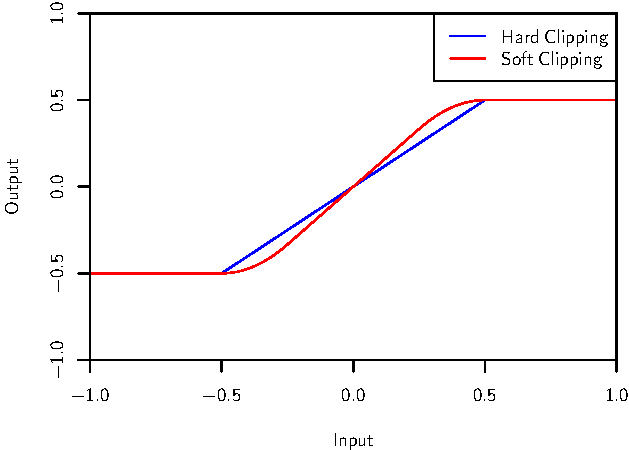
\includegraphics{chapter3/Images/Clipping.pdf}
			\caption{Characteristic curves for Equations \ref{eq:SymmetricHardClipping} and
				 \ref{eq:SymmetricSoftClipping} with a threshold of 0.5.}
			\label{fig:Clipping}
		\end{figure}

	\subsection{Rectification}
	\label{sec:Excitation-Methods-Rectification}
		Rectification is a special case of static nonlinearity based on analogue methods of producing a unipolar
		signal from a bipolar one. Half wave rectification (Equation~\ref{eq:HalfWaveRectification}) does so by
		zeroing any negative portions of the input signal, while full wave rectification
		(Equation~\ref{eq:FullWaveRectification}) inverts the polarity of negative portions of the input.

		\begin{equation}
			y[n] = \begin{cases}
				0 & \text{if $x[n] < 0$} \\
				x[n] & \text{otherwise}
			\end{cases}
			\label{eq:HalfWaveRectification}
		\end{equation}

		\begin{equation}
			y[n] = \abs{x[n]}
			\label{eq:FullWaveRectification}
		\end{equation}

	\subsection{Integrator}
	\label{sec:Excitation-Methods-Integrator}
		An integrator introduces new spectral content by integrating the input signal. \citet{larsen2004audio}
		describe an integrator which integrates the input signal after full wave rectification
		(Equation~\ref{eq:Integrator}).

		\begin{equation}
			y[n] = \begin{cases}
				0 & \text{if $x[n] > 0$ and $x[n - 1] \leq 0$} \\
				y[n - 1] + k\abs{x[n]} & \text{otherwise}
			\end{cases}
			\label{eq:Integrator}
		\end{equation}

		where $k$ is the integration constant, effectively setting the output gain of the system. The output signal
		is reset to zero after every negative to positive zero crossing in order to prevent the sample amplitudes
		from rising indefinitely. For periodic input signals, zeroing the output only on negative to positive zero
		crossings produces a signal with the same period as the input.

	\subsection{Multiplier}
	\label{sec:Excitation-Methods-Multiplier}
		Multipliers are a subset of static nonlinearities which apply automodulation to a signal. Automodulation
		refers to the amplitude modulation of a signal by itself. In amplitude modulation, the amplitude of one
		signal (the carrier) is varied according to another signal (the modulator) by multiplication,
		automodulation then refers to multiplying a signal by itself. The concept of automodulation can be extended
		by multiplying a signal by itself several times. This is achieved by raising input samples to a positive
		integer power, $h$, as shown in Equation~\ref{eq:Multiplier}.

		\begin{equation}
			y[n] = x^{h}[n], \quad h \in \textbf{N}
			\label{eq:Multiplier}
		\end{equation}

		To be considered a multiplier, a system in which the input signal is multiplied by itself, the restriction
		that $h$ be a positive integer ($h \in \textbf{N}$) must hold. If this restriction is relaxed to allow $h$
		to take any positive value ($h > 0$) the resulting system is referred to as an exponential static
		nonlinearity.

	\subsection{\acrlong{ssba}}
	\label{sec:Excitation-Methods-SSBA}
		\acrfull{ssba} combines the automodulation performed in a multiplier with the technique of single sideband
		modulation \citep{corinthios2009signals}. Regular amplitude modulation produces two sidebands (a sum and
		difference sideband) containing frequency components at the sums and differences in frequency of those in
		the carrier and modulator signals. Single sideband modulation is a method of applying amplitude modulation
		to a signal and only producing either the sum or difference sideband. This requires the construction of an
		analytic representation, $x_{a}[n]$, of the input signal, $x[n]$, as discussed in
		Section~\ref{sec:Timbre-LowLevelFeatures-Temporal}. The analytic signal is then raised to a positive
		integer power, $h$, as shown in Equation~\ref{eq:SSB}. Taking the real part of the resultant complex valued
		signal gives only the sum sideband of the modulation.

		\begin{equation}
			y[n] = \Re \left( x_{a}^{h}[n] \right), \quad h \in \textbf{N}
			\label{eq:SSB}
		\end{equation}

		The generation of only a single sideband can be illustrated by considering a sinusoidal input $\cos(x)$.
		Simply squaring the input produces two frequency components which are the sum and difference of the input's
		frequency and itself. These sum and difference sidebands are a sinusoid with twice the frequency of the
		input and a DC offset (0Hz) as seen in Equation~\ref{eq:TwoSidebands}.

		\begin{equation}
			\cos^{2}(x) = 0.5 + 0.5 \cos(2x)
			\label{eq:TwoSidebands}
		\end{equation}

		The analytic representation of our input signal is $\cos(x) + i\sin(x)$. Using De Moivre's formula it can
		be shown that squaring this signal and taking the real part only produces the sum sideband (the signal with
		twice the frequency). This is shown in Equation~\ref{eq:OneSideband}.

		\begin{equation}
			\bigl( \cos(x) + i\sin(x) \bigr)^{2} = \cos(2x) + i\sin(2x)
			\label{eq:OneSideband}
		\end{equation}

		With more thorough analysis it can be shown that the frequencies of intermodulation components produced
		through single sideband modulation all take the form shown in Equation~\ref{eq:IntermodulationComponents}
		but where the scaling factors, $k_{n}$, are all positive integers.

	\subsection{\acrlong{iap}}
	\label{sec:Excitation-Methods-IAP}
		In this method, the \acrfull{iap} of a signal are calculated from its analytic representation. These values
		are then used to aid in the construction of harmonics as discussed by \citet{puckette2007patch}. The
		instantaneous amplitude of the analytic signal is found by taking its absolute value, $\abs{x_{a}[n]}$. The
		instantaneous phase is found by taking the complex argument of the analytic signal, $\arg(x_{a}[n])$. The
		instantaneous phase can then be scaled in order to scale the frequency content of the signal independently
		of its amplitude.  Equation~\ref{eq:IAP} shows the $h$\super{th} order instantaneous amplitude and phase
		modulation of a signal.

		\begin{equation}
			y[n] = \abs{x_{a}[n]} \cos \bigl( h\arg \left( x_{a}[n] \right) \bigr), \quad h \in \textbf{N}
			\label{eq:IAP}
		\end{equation}

	\subsection{Spectral Replication}
	\label{sec:Excitation-Methods-SpectralReplication}
		Spectral replication is a method proposed for use in audio bandwidth extension applications
		\citep{nagel2010a}. The principle behind spectral replication is to reproduce the spectral structure of a
		signal at higher frequencies as shown in Figure~\ref{fig:SpectralReplication}.

		\begin{figure}[h!]
			\centering
			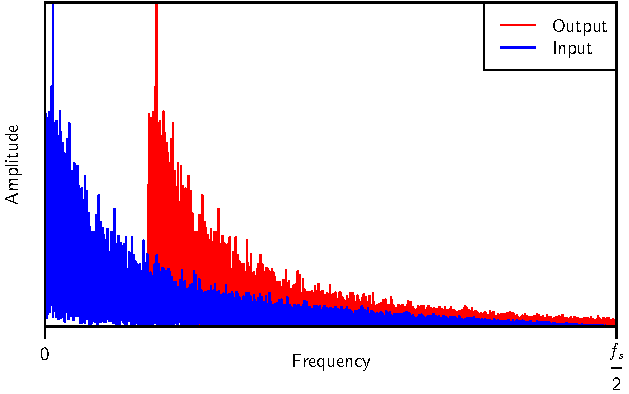
\includegraphics{chapter3/Images/SpectralReplicationSpectrum.pdf}
			\caption{Spectral reproduction of a signal at higher frequencies.}
			\label{fig:SpectralReplication}
		\end{figure}

		This shift of energy towards higher frequencies could be adapted for use in harmonic excitation systems.
		Shifting the spectrum $f$Hz higher in frequency is easily implemented through the use of single sideband
		modulation with a complex sinusoid as shown in Equation~\ref{eq:SpectralReplication}.

		\begin{equation}
			y[n] = \Re \left( x_{a}[n] e^{\frac{2i\pi fn}{f_{s}}} \right)
			\label{eq:SpectralReplication}
		\end{equation}

	\subsection{Spectral Folding}
	\label{sec:Excitation-Methods-SpectralFolding}
		Spectral folding is another method used in bandwidth extension \citep{friedrich2007spectral} which could be
		adapted for harmonic excitation. Spectral folding uses upsampling in order to replicate parts of the
		spectrum at higher frequencies. In order for the output signal to have the same sampling frequency as the
		input, the signal is downsampled by a factor $k$ before being upsampled by the same factor. To avoid
		aliasing during the downsampling phase, the signal should have a low pass filter applied with a cutoff
		frequency of $\frac{f_{s}}{2k}$. Typically upsampling systems apply a low pass filter to remove any high
		frequency content introduced \citep{oppenheim2014discrete}. This is not needed for spectral folding as the
		production of high frequency energy is the desired result. After low pass filtering, the downsampling and
		upsampling can be performed at the same time by retaining every $k$\super{th} sample and setting all others
		to zero. This is shown in Equation~\ref{eq:SpectralFolding}, where $x_{lf}[n]$ is the low pass filtered
		input signal.

		\begin{equation}
			y[n] = \begin{cases}
				x_{lf}[n] & \text{if $k \divides n$} \\
				0 & \text{otherwise}
			\end{cases}
			\label{eq:SpectralFolding}
		\end{equation}

		The effects of spectral folding with $k = 2$ and $k = 3$ are shown in Figure~\ref{fig:SpectralFolding}.

		\begin{figure}[h!]
			\centering
			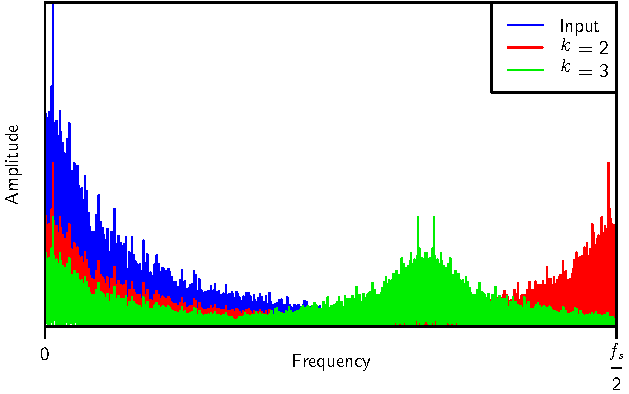
\includegraphics{chapter3/Images/SpectralFoldingSpectrum.pdf}
			\caption{The spectral characteristics of spectral folding.}
			\label{fig:SpectralFolding}
		\end{figure}

	\subsection{Spectral Stretching}
	\label{sec:Excitation-Methods-SpectralStretching}
		\citet{nagel2009a} propose spectral stretching as a bandwidth extension method. As with other bandwidth
		extension techniques it is possible to adapt for harmonic excitation purposes .The principle of spectral
		stretching is to scale the spectrum of a signal along the frequency axis. This effect is shown in
		Figure~\ref{fig:SpectralStretching}.

		\begin{figure}[h!]
			\centering
			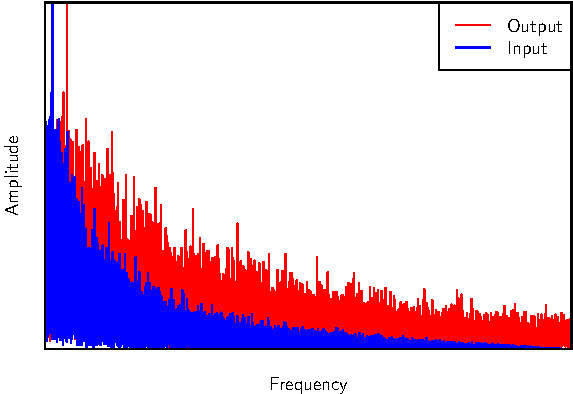
\includegraphics{chapter3/Images/SpectralStretchingSpectrum.pdf}
			\caption{The spectral characteristics of spectral stretching.}
			\label{fig:SpectralStretching}
		\end{figure}

		A typical implementation of this effect utilises a phase vocoder. The phase vocoder is an algorithm which
		allows for time stretching of a signal. It is applied by calculating the \acrfull{stft} of a signal with a
		given frame and hop size. The signal is then resynthesised using a different hop size in order to either
		lengthen or shorten it. This signal can then be resampled back to the length of the original signal,
		scaling the frequency content in the process. The spectrum is scaled by a factor, $s$, given by
		Equation~\ref{eq:PhaseVocoderFactor}.

		\begin{equation}
			s = \frac{\delta_{s}}{\delta_{a}}
			\label{eq:PhaseVocoderFactor}
		\end{equation}

		where $\delta_{a}$ is the hop size used when calculating the \acrshort{stft} and $\delta_{s}$ is the hop
		size used to resynthesise the signal.

	\subsection{\acrlong{sttr}}
	\label{sec:Excitation-Methods-STTR}
		\acrfull{sttr} is an audio effect proposed by \citet{kim2014shorttime}. The output signal is constructed by
		summing overlapping frames of the input signal which have been reversed in time using
		Equation~\ref{eq:STTR}, where $\delta$ is the step size between frames in samples and $w$ is an arbitrary
		window function which exhibits constant overlap add (i.e. the sum of the window function translated in time
		by all integer multiples of $\delta$ is equal to 1 at all values of $n$
		(Equation~\ref{eq:ConstantOverlapAdd})).  Constant overlap add ensures that no unwanted amplitude
		modulation is applied to the signal.

		\begin{equation}
			y[n] = \sum_{m = -\infty}^{\infty} w[n - m\delta]x[2m\delta - n]
			\label{eq:STTR}
		\end{equation}

		\begin{equation}
			\sum_{m = -\infty}^{\infty} w[n - m\delta] = 1
			\label{eq:ConstantOverlapAdd}
		\end{equation}

\section{Summary}
\label{sec:Excitation-Summary}
	In this chapter it has been shown that nonlinear systems find several uses within the audio processing field. Not
	only are they used as creative tools for timbral shaping but they can be used for corrective / reconstructive
	purposes. A number of nonlinear processing algorithms taken from implementations in these fields have been
	presented. The behaviour of such systems has been researched extensively both from the point of view of minimising
	audible distortion in audio processing equipment and modelling their nonlinear characteristics. Only more recently
	has research been carried out into the use of nonlinear distortion as a creative tool. In this area, publications
	have typically focussed on the application of distortion in specific use cases (the use of distortion pedals by
	guitar players \citep{tsumoto2016the}, the use of the Aphex Aural Exciter \citep{shekar2013modeling}) or have
	looked at the properties of distortion present in already recorded media \citep{wilson2014characterisation}. There
	is need for new research into the application of nonlinear distortion for creative purposes in order to generate
	semantically controlled distortion effects. In the following chapter the collection and analysis of data relating
	to this is discussed, providing the relevant data for the construction of these systems in subsequent chapters.
